%%%%%%%%%%%%%%%%%%%%%%%%%%%%%%%%%%%%%%%%%%%%%%%%%%%%%%%%%%%%%%%%%%%%%%%%%%%%%%%
% CHAPTER 16: EFFEKTIVE WAHRSCHEINLICHKEIT (P_eff)
% Frage 8: Wie gross ist die effektive Wahrscheinlichkeit, 
%          dass er/sie das Verhalten ändert?
%%%%%%%%%%%%%%%%%%%%%%%%%%%%%%%%%%%%%%%%%%%%%%%%%%%%%%%%%%%%%%%%%%%%%%%%%%%%%%%

% =============================================================================
% Chapter 16: Probability of Behavior Change
% =============================================================================
%
% Version: 1.0 (January 2026)
%
% Purpose: Effective probability output
%
% Primary Appendix: See appendix references below
% Secondary Appendices: G (Glossary), F (Examples)
%
% Prerequisites: Chapters 1-8 (Foundations)
% Leads to: Chapter 17
%
% Chapter Type: B (Foundation)
% =============================================================================


\chapter{Effective Probability of Behavioral Change: The Output}
\label{ch:peff}

%%%%%%%%%%%%%%%%%%%%%%%%%%%%%%%%%%%%%%%%%%%%%%%%%%%%%%%%%%%%%%%%%%%%%%%%%%%%%%%
% CHAPTER SCOPE BOX
%%%%%%%%%%%%%%%%%%%%%%%%%%%%%%%%%%%%%%%%%%%%%%%%%%%%%%%%%%%%%%%%%%%%%%%%%%%%%%%
\begin{tcolorbox}[
    colback=purple!5!white,
    colframe=purple!75!black,
    title={\textbf{Chapter Scope: Ziel / In-Scope / Out-of-Scope}},
    fonttitle=\bfseries
]

\textbf{Ziel (Objective):}
Develop the conceptual understanding of effective probability output as a foundation for the EBF framework.

\vspace{0.3cm}
\textbf{In-Scope:}
\begin{itemize}[nosep]
    \item Conceptual introduction to effective probability output
    \item Motivation and intuition
    \item Connection to subsequent chapters
    \item Key definitions and concepts
\end{itemize}

\vspace{0.3cm}
\textbf{Out-of-Scope (delegiert an Appendices):}
\begin{itemize}[nosep]
    \item Complete formal treatment $\rightarrow$ FORMAL appendices
    \item Empirical validation $\rightarrow$ METHOD appendices
    \item Domain applications $\rightarrow$ Application chapters
\end{itemize}

\end{tcolorbox}



%%%%%%%%%%%%%%%%%%%%%%%%%%%%%%%%%%%%%%%%%%%%%%%%%%%%%%%%%%%%%%%%%%%%%%%%%%%%%%%
% APPENDIX REFERENCES BOX
%%%%%%%%%%%%%%%%%%%%%%%%%%%%%%%%%%%%%%%%%%%%%%%%%%%%%%%%%%%%%%%%%%%%%%%%%%%%%%%
\begin{tcolorbox}[
    colback=yellow!10!white,
    colframe=orange!75!black,
    title={\textbf{Appendix References for This Chapter}},
    fonttitle=\bfseries
]
\small
\begin{tabular}{@{}lp{8cm}@{}}
\textbf{Appendix} & \textbf{Content} \\
\midrule
G (REF-GLOSSARY) & Symbol definitions and terminology \\
F (REF-EXAMPLES) & Additional worked examples \\
\end{tabular}

\medskip
\textit{For formal proofs and complete derivations, see the referenced appendices.}
\end{tcolorbox}

%%%%%%%%%%%%%%%%%%%%%%%%%%%%%%%%%%%%%%%%%%%%%%%%%%%%%%%%%%%%%%%%%%%%%%%%%%%%%%%
% CROSS-REFERENCE: EMERGE ALGORITHM (Chapter 11, EIT-EMP)
%%%%%%%%%%%%%%%%%%%%%%%%%%%%%%%%%%%%%%%%%%%%%%%%%%%%%%%%%%%%%%%%%%%%%%%%%%%%%%%
\begin{tcolorbox}[colback=blue!5!white, colframe=blue!75!black,
    title=\textbf{Cross-Reference: $P_{eff}$ als Input für EMERGE (Chapter 11, 17-22)}]

Die Berechnung von $P_{eff}$ in diesem Kapitel ist der \textbf{erste Schritt} vor dem EMERGE-Algorithmus (Kapitel 11, EIT-EMP):

\vspace{0.2cm}
\textbf{Workflow:}
\begin{center}
\small
Ch16 ($P_{eff}$, $S_0$) $\rightarrow$ Ch11 (EMERGE, $K^*$) $\rightarrow$ Ch17-22 (Interventions, Portfolios)
\end{center}

\textbf{$P_{eff}$ informiert K*-Faktoren (EIT-EMP-2):}
\begin{itemize}[nosep]
\item \textbf{$f_C$ (Complexity):} $1 - P_{eff,\text{base}}$ — niedriges $P_{eff}$ $\to$ komplexere Aufgabe $\to$ fokussierteres Portfolio
\item \textbf{$f_S$ (Stage):} $\alpha_{BCJ}$ aus Segment×Journey Matrix — Phase bestimmt K* Adjustment
\item \textbf{Scope-Level:} $P_{eff} < 0.2$ $\to$ L0/L1 (systemische Interventionen nötig)
\end{itemize}

\vspace{0.2cm}
\textbf{Diagnose-Output für EMERGE:}
\begin{equation*}
S_0 = (P_{eff}, \varphi, \text{segment}, \Psi) \quad \rightarrow \quad K^* = f(S_0)
\end{equation*}

\vspace{0.2cm}
\textit{Siehe: Chapter 11 §11.20 (EMERGE Algorithm), Chapter 17-22 (Intervention Design)}
\end{tcolorbox}

%%%%%%%%%%%%%%%%%%%%%%%%%%%%%%%%%%%%%%%%%%%%%%%%%%%%%%%%%%%%%%%%%%%%%%%%%%%%%%%
% INTUITION BOX
%%%%%%%%%%%%%%%%%%%%%%%%%%%%%%%%%%%%%%%%%%%%%%%%%%%%%%%%%%%%%%%%%%%%%%%%%%%%%%%
\begin{tcolorbox}[
    colback=blue!5!white,
    colframe=blue!75!black,
    title={\textbf{Intuition: A Motivating Example}},
    fonttitle=\bfseries
]
Consider \textbf{Anna}, a professional facing a decision that involves effective probability output.

She initially evaluates the choice using standard criteria, but something feels incomplete.
\textbf{Thomas}, her colleague, suggests considering additional dimensions beyond the obvious.

This chapter explores what Anna discovers when she applies the EBF framework---how
effective probability output interact with broader welfare considerations.

\medskip
\textit{By the end of this chapter, you will understand why Anna's initial analysis
was incomplete and how the EBF approach provides a more comprehensive view.}
\end{tcolorbox}



%------------------------------------------------------------------------------
% DIE 9 FRAGEN NAVIGATION BOX
%------------------------------------------------------------------------------
\BCMQuestionNav{16}

%------------------------------------------------------------------------------
% READING PATH FROM CHAPTER 15
%------------------------------------------------------------------------------

\begin{tcolorbox}[colback=blue!10!white, colframe=blue!75!black, title=Reading Path: From Chapter 15 (HI CORE-HIERARCHY)]

\textbf{You are here:} Chapter 16 (Probability of Behavioral Change) - The final output of the EBF framework.

\textbf{Coming from:} Chapter 15 (Decision Hierarchy \& Coherent Intervention Design) showed **HOW** to structure coherent interventions using the HI CORE-HIERARCHY and WEC (Willingness, Expectation, Compatibility) framework.

\textbf{In this chapter:} We answer: **GIVEN that your intervention is WEC-coherent, what is the probability that it actually changes behavior?**

\textbf{The Connection:} Chapter 15 ensures your intervention is coherent (all L2 decisions aligned). Chapter 16 calculates the probability that coherence translates to actual behavior change via the master equation: $P_{eff} = \sigma(WEC \cdot \alpha_{BCJ} \cdot \beta_{BCS})$

\textbf{Key insight:} Good design (Chapter 15) is necessary but not sufficient. Probability depends on how far the person is from the behavior threshold---Chapter 16 quantifies this.

\end{tcolorbox}

%------------------------------------------------------------------------------
% METADATA & QUICK REFERENCE
%------------------------------------------------------------------------------

\begin{tcolorbox}[colback=gray!10!white, colframe=gray!75!black, title=Chapter Metadata]
\begin{tabular}{@{}ll@{}}
\textbf{Type:} & Application Chapter (C) \\
\textbf{Version:} & 2.0 (January 2026) \\
\textbf{Purpose:} & Calculate and apply behavioral probability predictions \\
\textbf{Primary Appendix:} & PBB (FORMAL-PROBABILITY) - 10-axiom foundation \\
\textbf{UNTCM Appendix:} & UN (FORMAL-UNTCM) - Unified NTM-Context dynamics \\
\textbf{Secondary Appendices:} & BA, BB, AV, AW, C, AU, V, HI \\
\textbf{Prerequisite Chapters:} & Ch1-15, especially Ch13-15 \\
\textbf{Leads to:} & Ch17 (Policy Applications) \\
\end{tabular}
\end{tcolorbox}

\begin{tcolorbox}[colback=yellow!5!white, colframe=yellow!75!black, title=Quick Reference: In 60 Seconds]
\textbf{The Question:} Given a person's profile (utility, willingness, awareness, segment, journey stage, context), what is the probability they will change behavior?

\textbf{The Answer:} Calculate effective probability using:
\[\boxed{P_{eff} = \sigma(\text{WEC} \times \alpha_{BCJ} \times \beta_{BCS})}\]

\textbf{Three applications:}
1. \textbf{Lever Analysis} — Which variable matters most? (Willingness >> Awareness >> Context)
2. \textbf{Decision Tree} — Which intervention matches current P_eff? (Blockade/Incentive/Commitment/Maintain)
3. \textbf{Sensitivity} — How robust are predictions? (Segment classification is critical; context is robust)

\textbf{Practical use:} Predict outcome, monitor divergence from reality, diagnose failures, iterate. See Section~\ref{sec:ch16-monitoring} for 4-step adjustment protocol.
\end{tcolorbox}

%------------------------------------------------------------------------------
% CENTRAL QUESTION
%------------------------------------------------------------------------------

\begin{tcolorbox}[colback=red!10!white, colframe=red!75!black, title=Central Question of Chapter 16]
\textbf{The Probability Question (Question 8 of 9 in EBF):}

\Large\textbf{\textit{Given that we have diagnosed WHO (segments, Ch14), WHAT they value (utility, Ch10), HOW they're motivated (willingness, Ch12), WHEN they're ready (journey, Ch13), and HOW we coordinate the intervention (hierarchy, Ch15)---\\[8pt]what is the effective probability they actually change behavior?}}

\end{tcolorbox}

%------------------------------------------------------------------------------
% METHODOLOGICAL NOTE: EXCLUSION PRINCIPLE
%------------------------------------------------------------------------------
\begin{tcolorbox}[colback=red!5!white, colframe=red!75!black,
    title=\textbf{Methodological Note: The Exclusion Principle (Appendix FRM)}]
\textbf{Following Appendix FRM (LIT-FEHR-METHOD):}

This chapter's master equation combines multiple CORE components multiplicatively: $P_{eff} = \sigma(WEC \cdot \alpha_{BCJ} \cdot \beta_{BCS})$. Following the \textbf{Exclusion Principle}:
\begin{itemize}[nosep]
    \item \textbf{Null Hypothesis:} Components interact additively ($\gamma = 0$)
    \item \textbf{Alternative:} Non-additive interactions exist ($\gamma \neq 0$)
    \item \textbf{Empirical Requirement:} The multiplicative factors $\alpha_{BCJ}$ and $\beta_{BCS}$ must be empirically validated
\end{itemize}

\textbf{Practical implication:}
\begin{itemize}[nosep]
    \item Test whether additive probability $P = \sigma(WEC + BCJ + BCS)$ works first
    \item Only claim multiplicative interactions if additive model systematically fails
    \item Each interaction term must survive parameter perturbation (see Section~\ref{sec:ch16-sensitivity})
\end{itemize}
\end{tcolorbox}

%------------------------------------------------------------------------------
% CHAPTER OVERVIEW
%------------------------------------------------------------------------------

\section*{Chapter Overview: Five Sections}

This chapter is organized around five practical applications of behavioral probability:

\begin{enumerate}[label=\textbf{\arabic*.}]

\item \textbf{Introduction \& Master Equation} (Sections~\ref{sec:ch16-intro}--\ref{sec:ch16-model})
   — Formal probability architecture and complete formula

\item \textbf{Intervention Lever Analysis} (Section~\ref{sec:ch16-levers})
   — Identify which variable has highest impact via partial derivatives; practical example with Anna

\item \textbf{Segment × Journey Interaction Matrix} (Section~\ref{sec:ch16-matrix})
   — Heterogeneous probabilities across 4 segments × 6 journey stages; population-level implications

\item \textbf{Decision Tree \& Sensitivity Analysis} (Sections~\ref{sec:ch16-tree}--\ref{sec:ch16-sensitivity})
   — IF-THEN intervention selection; robustness of predictions under parameter changes

\item \textbf{Monitoring \& Adjustment Protocol} (Section~\ref{sec:ch16-monitoring})
   — 4-step feedback loop when predictions diverge from observed outcomes; implements Axiom P7 (Learning)

\end{enumerate}

\textbf{Reading paths:}
\begin{itemize}[nosep]
   \item \textbf{Quick practitioner:} Read Introduction + Decision Tree + Monitoring Protocol (~20 min)
   \item \textbf{Complete analysis:} Read all sections including UNTCM dynamics (~90 min)
   \item \textbf{Theory focus:} Read Introduction + Appendix PBB (axioms P1-P10) + Appendix UN (UNTCM dynamics)
\end{itemize}

%------------------------------------------------------------------------------
\section{Introduction: The Final Output}\label{sec:ch16-intro}
%------------------------------------------------------------------------------

This chapter answers the ultimate question of the EBF framework:

\begin{center}
\fbox{\parbox{0.85\textwidth}{
\textbf{Question 8:} How large is the \textbf{effective probability} 
that the person changes their behavior?
}}
\end{center}

All previous chapters have built toward this single output:

\begin{equation}
\boxed{P_{eff} = \sigma(WEC)}
\end{equation}

where $\sigma$ is the sigmoid function that maps WEC to a probability.

\textbf{Formal Foundation:} The complete axiomatization of the probabilistic framework appears in two appendices:
\begin{itemize}[nosep]
\item \textbf{Appendix PBB (FORMAL-PROBABILITY):} 10 axioms (P1-P10) formalizing how all BCM components integrate into transition probabilities; NTM basics (A1-A4, T1-T5)
\item \textbf{Appendix UN (FORMAL-UNTCM):} Unified NTM-Context Model with 29 elements---coupled ODE system, three regimes, tipping points, optimal timing, maintenance cost analysis, portfolio archetypes
\end{itemize}

%------------------------------------------------------------------------------
\section{The Complete EBF Model}\label{sec:ch16-model}
%------------------------------------------------------------------------------

\subsection{The Full Chain}

\begin{enumerate}
    \item \textbf{Context} ($\Psi$): Chapter 6
    \item \textbf{Utility} ($U$): Chapter 10
    \item \textbf{Awareness} ($AWX$): Chapter 11
    \item \textbf{Mindset} ($\varphi$): Chapter 12
    \item \textbf{Willingness} ($WAX$, $\theta$): Chapter 12
    \item \textbf{Journey} ($BCJ$): Chapter 13
    \item \textbf{Segment} ($BCS$): Chapter 14
    \item \textbf{Effective Willingness} ($WEC$): Chapter 15
    \item \textbf{Effective Probability} ($P_{eff}$): This Chapter
\end{enumerate}

\subsection{The Master Equation}

\begin{equation}
P_{eff} = \sigma\left( 
    \underbrace{
        \left[
            \underbrace{\varphi \cdot \min\{AWX \cdot U\} + (1-\varphi) \cdot \sum AWX \cdot U}_{WAX}
            - \underbrace{\theta_{base} + \sum \delta_j \Psi_j}_{\theta}
        \right]
    }_{WAX - \theta}
    \cdot \alpha_{BCJ} \cdot \beta_{BCS}
\right)
\end{equation}

where:
\begin{align}
\varphi &= \varphi_0 + \sum \gamma_j \Psi_j & \text{(Context-modulated mindset)} \\
U &= \{U_{INU}, U_{KNU}, U_{IDU}\} & \text{(Three-dimensional utility)} \\
AWX &\in [0,1] & \text{(Awareness function)} \\
\theta &= \theta_{base} + \sum \delta_j \Psi_j & \text{(Context-modulated threshold)} \\
\alpha_{BCJ} &\in (0,1] & \text{(Journey stage factor)} \\
\beta_{BCS} &\in (0.5, 1.2) & \text{(Segment type factor)}
\end{align}

%------------------------------------------------------------------------------
\section{The Sigmoid Transformation}
%------------------------------------------------------------------------------

\subsection{Definition}

\begin{equation}
\sigma(x) = \frac{1}{1 + e^{-kx}}
\end{equation}

where $k$ is a steepness parameter (default $k = 1$).

\subsection{Properties}

\begin{itemize}
    \item $\sigma(0) = 0.5$ — At the threshold, 50\% probability
    \item $\sigma(x) \rightarrow 1$ as $x \rightarrow \infty$
    \item $\sigma(x) \rightarrow 0$ as $x \rightarrow -\infty$
    \item Smooth transition around the threshold
\end{itemize}

\subsection{Interpretation}

\begin{center}
\begin{tabular}{rcl}
$WEC < 0$ & $\Rightarrow$ & $P_{eff} < 50\%$ — unlikely to act \\
$WEC = 0$ & $\Rightarrow$ & $P_{eff} = 50\%$ — indifferent \\
$WEC > 0$ & $\Rightarrow$ & $P_{eff} > 50\%$ — likely to act
\end{tabular}
\end{center}

%------------------------------------------------------------------------------
\section{Worked Example: Anna's Probability}
%------------------------------------------------------------------------------

\subsection{Baseline}

\begin{align}
WEC_{baseline} &= -0.50 \\
P_{eff,baseline} &= \sigma(-0.50) = \frac{1}{1 + e^{0.50}} \approx 0.38 = 38\%
\end{align}

\textbf{Interpretation:} Without intervention, Anna has only a 38\% probability 
of installing a heat pump.

\subsection{After Intervention}

\begin{align}
WEC_{intervention} &= +0.14 \\
P_{eff,intervention} &= \sigma(0.14) = \frac{1}{1 + e^{-0.14}} \approx 0.54 = 54\%
\end{align}

\textbf{Interpretation:} After intervention, Anna has a 54\% probability 
of installing a heat pump.

\subsection{The Intervention Effect}

\begin{equation}
\Delta P_{eff} = P_{eff,intervention} - P_{eff,baseline} = 54\% - 38\% = +16\%
\end{equation}

The intervention increased Anna's probability of behavioral change by
\textbf{16 percentage points}.

%------------------------------------------------------------------------------
\subsection{Natural Trajectory: What Happens Without Intervention?}
\label{sec:ch16-ntm}
%------------------------------------------------------------------------------

A critical question for intervention planning: \textbf{If we do nothing, how will Anna's probability evolve over time?}

The \textbf{Natural Trajectory Model (NTM)} from Appendix PBB formalizes basic decay dynamics, while the \textbf{Unified NTM-Context Model (UNTCM)} in \textbf{Appendix UN (FORMAL-UNTCM)} provides the complete coupled ODE system:

\begin{equation}
\vec{S}(t+\Delta t) = f_{NTM}(\vec{S}(t), \Psi(t), \Delta t, \mathbf{0})
\end{equation}

\textbf{Anna's Natural Trajectory (Without Intervention):}

\begin{center}
\renewcommand{\arraystretch}{1.3}
\begin{tabular}{@{}llll@{}}
\toprule
\textbf{Time Horizon} & \textbf{$\Delta t$} & \textbf{Key Changes} & \textbf{$P_{eff}$} \\
\midrule
\textbf{Instant} & $t = 0$ & Status quo: $A = 0.55$, $W = -0.50$ & 38\% \\
\textbf{Short-term} & 4 weeks & $A \downarrow$ to 0.42 (decay), habits reinforce & 31\% \\
\textbf{Medium-term} & 6 months & $A \downarrow$ to 0.25, $\theta \uparrow$, identity lock-in & 22\% \\
\textbf{Long-term} & 2 years & New equilibrium: ``Ich bin kein Wärmepumpen-Typ'' & 12\% \\
\bottomrule
\end{tabular}
\end{center}

\textbf{Interpretation:}
\begin{itemize}[nosep]
\item \textbf{Instant:} Anna's 38\% baseline is a snapshot, not a stable state
\item \textbf{Short-term:} Awareness decays (AWX-A58: $A(t) = A_0 \cdot e^{-\lambda t}$); probability drops by ~7pp
\item \textbf{Medium-term:} Procrastination accumulates ($\theta \uparrow$), identity crystallizes around non-action
\item \textbf{Long-term:} Path dependence locks in; ``So bin ich halt'' becomes self-fulfilling
\end{itemize}

\textbf{Intervention Necessity Criterion (NTM-T2):}

\begin{equation}
\text{Intervention Required} \Leftrightarrow P_{NTM}(t + \Delta t) < P_{target} - \epsilon
\end{equation}

For Anna: If our target is 50\% adoption probability, and NTM predicts decay to 22\% in 6 months, \textbf{intervention is urgent}. The gap widens over time, increasing intervention cost.

\textbf{Practical Implication:} Early intervention is cheaper than late intervention. The NTM quantifies the \textbf{cost of delay}.

%------------------------------------------------------------------------------
\subsection{UNTCM: The Unified NTM-Context Model}
\label{sec:ch16-untcm}
%------------------------------------------------------------------------------

The \textbf{Unified NTM-Context Model (UNTCM)} extends basic NTM with context modulation and social feedback. The complete formalization is in \textbf{Appendix UN (FORMAL-UNTCM)}.

\subsubsection{The Coupled ODE System}

UNTCM models three interdependent state variables:

\begin{align}
\frac{dA}{dt} &= -\lambda(\Psi) \cdot A + \kappa_A \cdot f(B) + I_A(t) \label{eq:untcm-A} \\
\frac{dW}{dt} &= -\mu(\Psi) \cdot W + \kappa_W \cdot g(B) + I_W(t) \label{eq:untcm-W} \\
\frac{dB}{dt} &= \alpha \cdot P(A, W, \theta) - \delta \cdot B \label{eq:untcm-B}
\end{align}

where:
\begin{itemize}[nosep]
\item $A$ = Awareness, $W$ = Willingness, $B$ = Behavioral adoption rate
\item $\lambda(\Psi), \mu(\Psi), \delta$ = Context-modulated decay rates
\item $\kappa_A, \kappa_W$ = Social feedback coefficients
\item $I_A(t), I_W(t)$ = Intervention inputs
\item $P(A, W, \theta)$ = Probability of crossing threshold
\end{itemize}

\subsubsection{The Three Regimes}

UNTCM identifies three dynamically distinct regimes (see Appendix UN, Section UNTCM-T7):

\begin{center}
\renewcommand{\arraystretch}{1.3}
\begin{tabular}{@{}llll@{}}
\toprule
\textbf{Regime} & \textbf{Condition} & \textbf{Behavior} & \textbf{Anna's Implication} \\
\midrule
\textbf{I: Decay-Dominant} & $\kappa < \kappa^*$ & Fades without intervention & Without intervention, $P_{eff} \to 12\%$ \\
\textbf{II: Feedback-Dominant} & $\kappa > \kappa^*$ & Self-sustaining lock-in & If neighbors adopt, $P_{eff} \to 75\%+$ \\
\textbf{III: Oscillatory} & Complex $\kappa$ & Cycles between high/low & Seasonal variation possible \\
\bottomrule
\end{tabular}
\end{center}

\textbf{Critical Insight:} The \textbf{tipping point} $\bar{B}^* \approx 10-25\%$ determines which regime the system enters. If neighborhood adoption exceeds ~25\%, Anna experiences social feedback that can trigger Regime II lock-in.

\subsubsection{Context Drift Effects}

UNTCM captures how decay rates change over time (UNTCM-A5):

\begin{equation}
\lambda(t) = \lambda_0 \cdot \left(1 + \sum_j \xi_j \cdot \Psi_j(t)\right)
\end{equation}

\textbf{For Anna:}
\begin{itemize}[nosep]
\item \textbf{Positive drift:} Rising energy prices ($\Psi_E \uparrow$) → decay slows ($\lambda \downarrow$), awareness persists longer
\item \textbf{Negative drift:} Policy uncertainty ($\Psi_I \downarrow$) → decay accelerates ($\lambda \uparrow$), awareness fades faster
\item \textbf{Social drift:} Neighbor adoption ($\Psi_S \uparrow$) → social feedback kicks in ($\kappa \uparrow$)
\end{itemize}

\subsubsection{Optimal Intervention Timing (UNTCM-T8)}

UNTCM provides a formal rule for optimal intervention timing:

\begin{equation}
t^* = \arg\max_t \left[ \Delta P_{eff}(t) - C(t) \right]
\end{equation}

\textbf{Key Finding:} Intervene \textbf{early in Regime I} (before decay accumulates) or \textbf{at the tipping point} (to trigger Regime II). Intervening mid-decay is least efficient.

\subsubsection{Status-Quo Lock-in via Loss Aversion (UNTCM-X5)}

A critical insight: \textbf{Why does the effective threshold $\theta_{eff}$ increase over time?}

UNTCM-X5 formalizes the connection between decay and loss aversion:

\begin{enumerate}[nosep]
\item \textbf{Reference Point Drift:} As time passes without action, the current state $S(t)$ becomes the psychological reference point $r(t)$
\item \textbf{Loss Framing:} Any proposed change from the status quo is now perceived as a \textbf{loss}
\item \textbf{Loss Aversion Amplification:} Losses are weighted $\lambda_{LA} \approx 2.25\times$ more than gains (Kahneman \& Tversky)
\end{enumerate}

\textbf{Mathematical Formulation:}
\begin{align}
\frac{dr}{dt} &= \eta_r \cdot (S(t) - r(t)) & \text{(Reference point drift)} \\
\theta_{eff}(t) &= \theta_0 + \lambda_{LA} \cdot |S_{target} - r(t)| & \text{(Effective threshold)}
\end{align}

\textbf{For Anna:} If she waits 6 months without acting, her reference point crystallizes around ``not having a heat pump.'' Now installing one feels like a \textit{loss} of her current comfortable status quo---even though objectively it's a gain. Her effective threshold has increased by $\approx 2.25 \times \Delta S$.

\textbf{Intervention Implication:} Late intervention requires either (a) much stronger incentives, or (b) \textbf{reference point reset} via temporal landmarks (Fresh Start Effect) or life events.

\subsubsection{Maintenance Cost Analysis (UNTCM-M5)}

A crucial question practitioners often overlook: \textbf{What does it cost to maintain the status quo?}

UNTCM-M5 (Appendix UN) formalizes the \textbf{Maintenance Paradox}: Status quo preservation is NOT free and becomes MORE expensive over time due to the X5 loss aversion premium.

\textbf{FEPSDE-Specific Decay Rates:}

Each utility dimension decays at different rates, requiring different maintenance interventions:

\begin{center}
\renewcommand{\arraystretch}{1.2}
\begin{tabular}{@{}lcll@{}}
\toprule
\textbf{Dimension} & \textbf{$\lambda_d$} & \textbf{Half-Life} & \textbf{Anna's Implication} \\
\midrule
Financial (F) & 0.02/wk & 35 weeks & Cost savings awareness persists \\
Emotional (E) & 0.15/wk & 4.6 weeks & Enthusiasm fades quickly \\
Physical (P) & 0.08/wk & 8.7 weeks & Comfort concerns moderate \\
Social (S) & 0.04/wk & 17 weeks & Neighbor influence stable \\
Developmental (D) & 0.01/wk & 69 weeks & Learning about heat pumps retained \\
Experiential (Ex) & 0.20/wk & 3.5 weeks & Showroom visit forgotten fastest \\
\bottomrule
\end{tabular}
\end{center}

\textbf{For Anna:} Her emotional excitement (E) from the energy consultant visit decays fastest ($t_{1/2} = 4.6$ weeks). If no follow-up within 5 weeks, her emotional engagement must be rebuilt from scratch---at 225\% cost due to X5 premium.

\textbf{The Maintenance Cost Function (M5):}

\begin{equation}
I_d^{maintain}(t) = \underbrace{\lambda_d \cdot U_d(0)}_{\text{Base decay}} + \underbrace{\lambda_{LA} \cdot \eta_r \cdot (1 - e^{-\eta_r t}) \cdot \Delta\theta_d}_{\text{X5 premium}}
\end{equation}

\textbf{Time Horizon Implications for Anna:}

\begin{center}
\renewcommand{\arraystretch}{1.3}
\begin{tabular}{@{}lcll@{}}
\toprule
\textbf{Horizon} & \textbf{X5 Premium} & \textbf{Required Intervention} & \textbf{Cost Index} \\
\midrule
Instant ($<$1 day) & $\approx 0$ & Follow-up call same day & 1.0$\times$ \\
Short (1-4 weeks) & 0.1-0.3$\times$ & Email reminder, brochure & 1.3$\times$ \\
Medium (1-6 months) & 0.5-1.0$\times$ & Second consultation, site visit & 2.0$\times$ \\
Long ($>$6 months) & 1.5-2.25$\times$ & Full re-engagement campaign & 3.25$\times$ \\
\bottomrule
\end{tabular}
\end{center}

\textbf{Theorem M5-T1 (Superlinearity):} Cumulative maintenance cost grows \emph{superlinearly}:
\begin{equation}
C_{maintain}(T) \approx (\lambda_d U_d(0) + \lambda_{LA} \Delta\theta_d) \cdot T - \frac{\lambda_{LA} \Delta\theta_d}{\eta_r}
\end{equation}

The asymptotic rate is $(1 + \lambda_{LA}) \approx 3.25\times$ the base cost---a 225\% premium for late intervention.

\textbf{Practical Implication for Anna's Case:}
\begin{itemize}[nosep]
\item \textbf{Optimal timing:} Follow up within 4 weeks (before E dimension decays)
\item \textbf{Cost of delay:} Waiting 6 months costs 3.25$\times$ the immediate intervention
\item \textbf{Fresh Start strategy:} If delayed, use New Year or spring (heating season end) as reference point reset
\item \textbf{Portfolio design:} Include maintenance touchpoints in Sustainable Archetype (Chapter 20)
\end{itemize}

\subsubsection{Minimal Maintenance Portfolio: The Status Quo Preservation Toolkit}

What is the \textbf{minimal intervention set} required to maintain utility levels across all FEPSDE dimensions and all three utility levels ($u_I$, $u_C$, $u_D$)?

\textbf{Intervention Types for Maintenance (from Chapter 17):}

\begin{center}
\renewcommand{\arraystretch}{1.2}
\begin{tabular}{@{}clll@{}}
\toprule
\textbf{10C Dim.} & \textbf{Name} & \textbf{Primary Target} & \textbf{Maintenance Role} \\
\midrule
AWARE & Awareness & $A(\cdot)$ & Refresh salience \\
READY & Feedback & $\kappa_{AWX}$ & Self-correction loops \\
WHEN & Contextual & $\kappa_{KON}$ & Environment optimization \\
STAGE & Temporal & $\kappa_{JNY}$ & Timing \& deadlines \\
WHO & Identity & $W_{base}$ & Value reinforcement \\
WHAT$_S$ & Social & $u_S$ & Norm maintenance \\
WHAT$_F$ & Financial & $u_F$ & Incentive continuation \\
HOW & Commitment & $\gamma_{ij}$ & Goal renewal \\
\bottomrule
\end{tabular}
\end{center}

\textbf{Minimal Maintenance Portfolio by Time Horizon:}

\begin{tcolorbox}[colback=green!5!white, colframe=green!75!black, title=Minimal Maintenance Portfolio: Time Horizon × Utility Level × FEPSDE]

\textbf{INSTANT ($<$ 1 day):} Prevent immediate decay
\begin{center}
\renewcommand{\arraystretch}{1.1}
\begin{tabular}{@{}llll@{}}
\toprule
\textbf{Utility} & \textbf{FEPSDE Focus} & \textbf{Intervention} & \textbf{Example (Anna)} \\
\midrule
$u_I$ & E, Ex & AWARE & Same-day follow-up call \\
$u_C$ & S & WHAT$_S$ (Social) & ``Your neighbor also inquired today'' \\
$u_D$ & D & WHO (Identity) & ``As someone who values sustainability...'' \\
\bottomrule
\end{tabular}
\end{center}

\textbf{SHORT-TERM (1-4 weeks):} Counteract fast-decay dimensions
\begin{center}
\renewcommand{\arraystretch}{1.1}
\begin{tabular}{@{}llll@{}}
\toprule
\textbf{Utility} & \textbf{FEPSDE Focus} & \textbf{Intervention} & \textbf{Example (Anna)} \\
\midrule
$u_I$ & E, Ex, P & READY (Feedback) & Progress tracker, energy cost app \\
$u_I$ & F & WHEN (Contextual) & Simplified financing brochure \\
$u_C$ & S & WHAT$_S$ (Social) & Neighborhood adoption update \\
$u_D$ & D & HOW (Commitment) & ``Reminder: You expressed interest on [date]'' \\
\bottomrule
\end{tabular}
\end{center}

\textbf{MEDIUM-TERM (1-6 months):} Rebuild decayed dimensions, counter X5 premium
\begin{center}
\renewcommand{\arraystretch}{1.1}
\begin{tabular}{@{}llll@{}}
\toprule
\textbf{Utility} & \textbf{FEPSDE Focus} & \textbf{Intervention} & \textbf{Example (Anna)} \\
\midrule
$u_I$ & E, Ex & AWARE + STAGE (Temporal) & Second consultation, seasonal deadline \\
$u_I$ & F, P & WHAT$_F$ (Financial) & Limited-time subsidy reminder \\
$u_C$ & S & WHAT$_S$ (Social) & Community workshop invitation \\
$u_D$ & D & WHO (Identity) & ``Families like yours are leading the transition'' \\
\bottomrule
\end{tabular}
\end{center}

\textbf{LONG-TERM ($>$ 6 months):} Full re-engagement, reference point reset required
\begin{center}
\renewcommand{\arraystretch}{1.1}
\begin{tabular}{@{}llll@{}}
\toprule
\textbf{Utility} & \textbf{FEPSDE Focus} & \textbf{Intervention} & \textbf{Example (Anna)} \\
\midrule
$u_I$ & All & AWARE + STAGE (Fresh Start) & New Year campaign, spring re-contact \\
$u_I$ & F & WHAT$_F$ (Financial) & New incentive program announcement \\
$u_C$ & S & WHAT$_S$ + AWARE & ``30\% of your street now has heat pumps'' \\
$u_D$ & D & WHO + HOW (Identity Reset) & Life event trigger (retirement, renovation) \\
\bottomrule
\end{tabular}
\end{center}

\end{tcolorbox}

\textbf{Minimal Portfolio Summary Table:}

\begin{center}
\renewcommand{\arraystretch}{1.3}
\begin{tabular}{@{}lp{7cm}c@{}}
\toprule
\textbf{Horizon} & \textbf{Emergent Intervention Emphasis}\footnotemark & \textbf{Min. Dimensions} \\
\midrule
Instant & AWARE + WHO + WHAT$_S$ & 3 \\
Short & AWARE + READY + WHEN + WHAT$_S$ + HOW & 5 \\
Medium & AWARE + STAGE + WHO + WHAT$_S$ + WHAT$_F$ & 5 \\
Long & AWARE + STAGE + WHO + WHAT$_S$ + WHAT$_F$ + HOW & 6 \\
\bottomrule
\end{tabular}
\end{center}
\footnotetext{Interventions \textit{emerge} from the continuous 10C space $[0,1]^9$ based on context analysis (Ch.~17, Axiom EIT-3). The emphases shown indicate which 10C dimensions should have high intensity in the emergent intervention vector $\vec{I}$.}

\textbf{Key Insights:}
\begin{itemize}[nosep]
\item \textbf{AWARE and WHAT$_S$ (Social)} are needed at \emph{every} horizon---they are the maintenance backbone
\item \textbf{WHO (Identity)} becomes critical from medium-term onwards---status quo threatens identity alignment
\item \textbf{WHAT$_F$ (Financial)} only needed medium+ when X5 premium requires stronger incentives
\item \textbf{HOW (Commitment)} needed at short (reminder) and long (renewal) horizons
\item \textbf{Minimal instant portfolio:} Just 3 emphases (AWARE, WHO, WHAT$_S$) can prevent immediate decay
\item \textbf{Long-term requires 6 dimensions:} The X5 premium demands a full toolkit
\end{itemize}

\textbf{Anna's Minimal Maintenance Schedule:}

\begin{center}
\renewcommand{\arraystretch}{1.2}
\begin{tabular}{@{}llll@{}}
\toprule
\textbf{When} & \textbf{Intervention} & \textbf{10C Emphasis} & \textbf{Cost Index} \\
\midrule
Day 0 & Consultant visit + identity framing & AWARE, WHO & 1.0$\times$ \\
Day 1 & Follow-up call + neighbor mention & AWARE, WHAT$_S$ & 1.0$\times$ \\
Week 2 & Energy cost tracker app & READY & 1.1$\times$ \\
Week 4 & Financing brochure + deadline & WHEN, STAGE & 1.3$\times$ \\
Month 3 & Community workshop & WHAT$_S$ & 1.7$\times$ \\
Month 6 & Subsidy deadline reminder & STAGE, WHAT$_F$ & 2.0$\times$ \\
Month 12 & New Year Fresh Start campaign & AWARE, STAGE, WHO, HOW & 3.25$\times$ \\
\bottomrule
\end{tabular}
\end{center}

\textbf{Total Maintenance Cost (12-month program):} $\sum = 11.35 \times$ base intervention cost

\textbf{Comparison:} A single intervention at month 12 (without prior maintenance) would cost $3.25\times$ but with much lower success probability due to full decay. The distributed maintenance approach costs more but \emph{maintains} $P_{eff}$ throughout.

%------------------------------------------------------------------------------
\subsubsection{Portfolio Archetypes for Maintenance: Beyond Minimal}
\label{sec:ch16-portfolio-archetypes}
%------------------------------------------------------------------------------

The Minimal Maintenance Portfolio (Section~\ref{sec:ch16-maintenance-portfolio}) answers: \textit{What is the smallest intervention set that prevents decay?} But practitioners often face different optimization objectives. We formalize \textbf{five Portfolio Archetypes} that span the Pareto-frontier between cost and effectiveness:

\begin{tcolorbox}[colback=purple!5!white, colframe=purple!75!black, title=Portfolio Archetype Definitions (M5-D2)]

\textbf{Definition M5-D2: Portfolio Archetypes for Maintenance}

Given time horizon $H$, let $\mathcal{P}$ be an intervention portfolio (a vector in $[0,1]^9$ specifying emphasis on each 10C dimension). We define five archetypes:

\begin{enumerate}[nosep]
\item \textbf{Minimal Portfolio} $\mathcal{P}^{min}$: Smallest $|\mathcal{P}|$ such that $\forall d: U_d(H) \geq U_d(0) - \epsilon$
\[
\mathcal{P}^{min}(H) = \arg\min_{\mathcal{P}} |\mathcal{P}| \quad \text{s.t. maintenance constraint}
\]

\item \textbf{Cost-Optimal Portfolio} $\mathcal{P}^{cost}$: Minimize total cost while maintaining all dimensions
\[
\mathcal{P}^{cost}(H) = \arg\min_{\mathcal{P}} \sum_{T_i \in \mathcal{P}} c_i(H) \quad \text{s.t. maintenance constraint}
\]

\item \textbf{Effectiveness-Optimal Portfolio} $\mathcal{P}^{eff}$: Maximize $P_{eff}$ gain per unit cost
\[
\mathcal{P}^{eff}(H) = \arg\max_{\mathcal{P}} \frac{\Delta P_{eff}(\mathcal{P})}{\sum_{T_i \in \mathcal{P}} c_i(H)}
\]

\item \textbf{Risk-Adjusted Portfolio} $\mathcal{P}^{risk}$: Minimize variance in maintenance success
\[
\mathcal{P}^{risk}(H) = \arg\min_{\mathcal{P}} \text{Var}[U_d(H) | \mathcal{P}] \quad \text{s.t. } \mathbb{E}[U_d(H)] \geq U_d(0) - \epsilon
\]

\item \textbf{Segment-Specific Portfolio} $\mathcal{P}^{seg}$: Apply segment multipliers $\sigma_s$ from Chapter 19
\[
\mathcal{P}^{seg}(H, s) = \arg\max_{\mathcal{P}} \sum_{T_i \in \mathcal{P}} \sigma_{s,i} \cdot \text{eff}_i(H)
\]
\end{enumerate}

\end{tcolorbox}

\textbf{Portfolio Archetype Comparison Table:}

\begin{center}
\renewcommand{\arraystretch}{1.3}
\begin{tabular}{@{}lcccc@{}}
\toprule
\textbf{Archetype} & \textbf{Optimizes} & \textbf{Typical Size} & \textbf{Cost Index} & \textbf{Risk Profile} \\
\midrule
Minimal ($\mathcal{P}^{min}$) & Cardinality & 3--6 & 1.0$\times$ & Medium \\
Cost-Optimal ($\mathcal{P}^{cost}$) & Total Cost & 4--5 & 0.85$\times$ & Medium-High \\
Effectiveness-Optimal ($\mathcal{P}^{eff}$) & ROI & 5--7 & 1.2$\times$ & Low \\
Risk-Adjusted ($\mathcal{P}^{risk}$) & Variance & 6--8 & 1.5$\times$ & Very Low \\
Segment-Specific ($\mathcal{P}^{seg}$) & Fit & Varies & 0.9--1.3$\times$ & Segment-dependent \\
\bottomrule
\end{tabular}
\end{center}

\begin{tcolorbox}[colback=green!5!white, colframe=green!75!black, title=The Pareto-Frontier: Cost vs. Effectiveness (M5-T3)]

\textbf{Theorem M5-T3: Maintenance Portfolio Pareto-Frontier}

For any time horizon $H$, the set of efficient portfolios forms a Pareto-frontier $\mathcal{F}(H)$ in Cost × Effectiveness space:

\[
\mathcal{F}(H) = \left\{ \mathcal{P} : \nexists \mathcal{P}' \text{ with } \text{Cost}(\mathcal{P}') \leq \text{Cost}(\mathcal{P}) \text{ and } \text{Eff}(\mathcal{P}') \geq \text{Eff}(\mathcal{P}) \right\}
\]

\textbf{Key Properties:}
\begin{itemize}[nosep]
\item $\mathcal{P}^{min} \in \mathcal{F}$ (minimal portfolio is Pareto-efficient)
\item $\mathcal{P}^{cost} \in \mathcal{F}$ (cost-optimal is Pareto-efficient)
\item $|\mathcal{F}(H)|$ increases with horizon $H$ (more trade-off options for longer horizons)
\item The frontier shifts \textit{outward} with X5 premium: longer horizons require more resources
\end{itemize}

\end{tcolorbox}

\textbf{Visual: Pareto-Frontier for 12-Month Maintenance}

\begin{center}
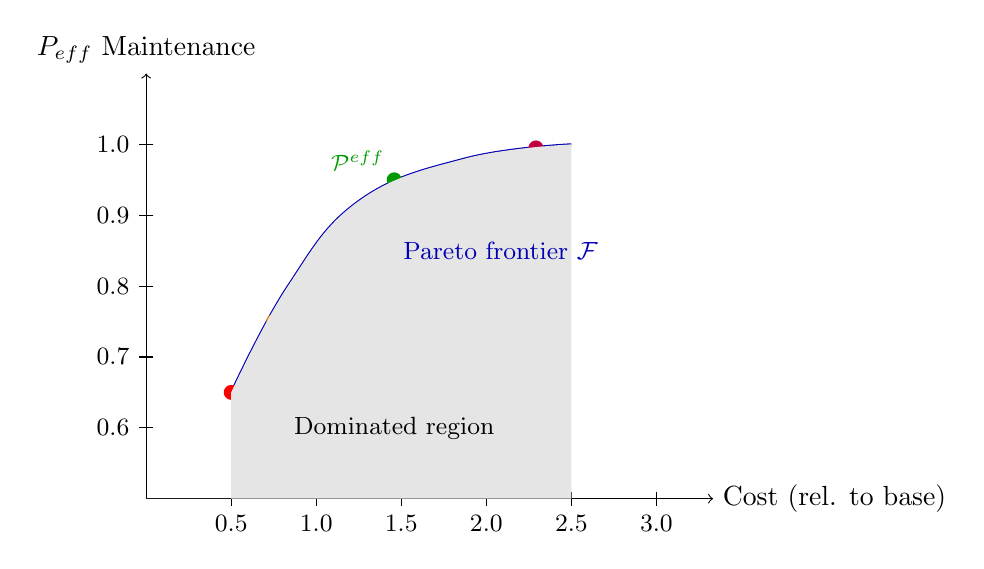
\begin{tikzpicture}[scale=0.9]
% Axes
\draw[->] (0,0) -- (8,0) node[right] {Cost (rel. to base)};
\draw[->] (0,0) -- (0,6) node[above] {$P_{eff}$ Maintenance};

% Axis labels
\foreach \x/\label in {1/0.5, 2/1.0, 3/1.5, 4/2.0, 5/2.5, 6/3.0}
    \draw (\x*1.2,0.1) -- (\x*1.2,-0.1) node[below] {\small \label};
\foreach \y/\label in {1/0.6, 2/0.7, 3/0.8, 4/0.9, 5/1.0}
    \draw (0.1,\y) -- (-0.1,\y) node[left] {\small \label};

% Pareto frontier (smooth curve)
\draw[thick, blue!70!black] plot[smooth, tension=0.7] coordinates {(1.2,1.5) (2,3) (3,4.2) (4.5,4.8) (6,5)};

% Portfolio points
\fill[red] (1.2,1.5) circle (3pt) node[below right] {\footnotesize $\mathcal{P}^{min}$};
\fill[orange] (1.8,2.5) circle (3pt) node[below right] {\footnotesize $\mathcal{P}^{cost}$};
\fill[green!60!black] (3.5,4.5) circle (3pt) node[above left] {\footnotesize $\mathcal{P}^{eff}$};
\fill[purple] (5.5,4.95) circle (3pt) node[below left] {\footnotesize $\mathcal{P}^{risk}$};

% Dominated region
\fill[gray!20] (0,0) -- (1.2,0) -- (1.2,1.5) -- plot[smooth, tension=0.7] coordinates {(1.2,1.5) (2,3) (3,4.2) (4.5,4.8) (6,5)} -- (6,0) -- cycle;

% Label
\node at (3.5,1) {\small Dominated region};
\node[blue!70!black] at (5,3.5) {\small Pareto frontier $\mathcal{F}$};
\end{tikzpicture}
\end{center}

\textbf{Portfolio Selection Decision Tree:}

\begin{center}
\renewcommand{\arraystretch}{1.3}
\begin{tabular}{@{}lll@{}}
\toprule
\textbf{Situation} & \textbf{Recommended Archetype} & \textbf{Rationale} \\
\midrule
Budget-constrained & $\mathcal{P}^{cost}$ & Minimize expenditure \\
Risk-averse stakeholder & $\mathcal{P}^{risk}$ & Reduce variance, even if costly \\
Maximizing ROI & $\mathcal{P}^{eff}$ & Best return per euro \\
Unknown segment & $\mathcal{P}^{min}$ & Safe default \\
Known high-multiplier segment & $\mathcal{P}^{seg}$ & Leverage segment fit \\
Short horizon (< 1 month) & $\mathcal{P}^{min}$ & Complexity not justified \\
Long horizon (> 6 months) & $\mathcal{P}^{risk}$ or $\mathcal{P}^{eff}$ & Worth investing in robustness \\
\bottomrule
\end{tabular}
\end{center}

\textbf{Anna's Portfolio Selection:}

For Anna (Pragmatist segment, 12-month horizon, moderate budget):
\begin{itemize}[nosep]
\item \textbf{Minimal Portfolio} ($\mathcal{P}^{min}$): 6 intervention types, Cost = 11.35$\times$, Risk = Medium
\item \textbf{Cost-Optimal} ($\mathcal{P}^{cost}$): 5 dimensions (drop WHAT$_F$), Cost = 9.8$\times$, Risk = Medium-High
\item \textbf{Effectiveness-Optimal} ($\mathcal{P}^{eff}$): 7 dimensions (add READY tracking), Cost = 13.5$\times$, Risk = Low
\item \textbf{Recommendation:} $\mathcal{P}^{eff}$ if utility company funds it; $\mathcal{P}^{cost}$ if self-funded
\end{itemize}

\textbf{Crowding-Out Warning (Chapter 20):} When combining WHAT$_S$ (Social) + WHAT$_F$ (Financial) in portfolios, monitor for crowding-out ($\gamma_{S,F} = -0.2$). Consider \textit{sequential deployment}: WHAT$_S$ first to establish norms, WHAT$_F$ later if needed.

\begin{tcolorbox}[colback=blue!5!white, colframe=blue!75!black, title=UNTCM Summary for Practitioners]
\textbf{Five questions UNTCM answers:}
\begin{enumerate}[nosep]
\item \textbf{What regime?} Diagnose whether decay-dominant (intervene early) or feedback-dominant (leverage social proof)
\item \textbf{Where is tipping point?} Estimate $\bar{B}^* \approx 10-25\%$; target early adopters to cross threshold
\item \textbf{When to intervene?} Use timing rule: early (prevent decay) or at tipping (trigger cascade)
\item \textbf{Why early matters:} Loss aversion amplifies status quo over time (X5); late intervention faces $\theta_{eff} \approx 2.25\times$ higher
\item \textbf{What does maintenance cost?} Status quo preservation grows superlinearly (M5); asymptotic cost is $3.25\times$ base rate
\end{enumerate}
\textbf{Full formalization:} Appendix UN (FORMAL-UNTCM) with 29 elements (A5, T6-T8, M1-M5, M5-D1/D2, M5-T2/T3, I1-I4, E1-E3, X1-X5).
\end{tcolorbox}

\begin{tcolorbox}[colback=orange!5!white, colframe=orange!75!black, title=UNTCM Connection to Portfolio Archetypes (Chapter 20)]
The UNTCM regime classification informs Portfolio Archetype selection:
\begin{itemize}[nosep]
\item \textbf{Regime I (Decay-Dominant)} → \textbf{Quick Wins Archetype}: Intervene before awareness/willingness fade
\item \textbf{Regime II (Feedback-Dominant)} → \textbf{Sustainable Archetype}: Leverage social feedback, invest in early adopters
\item \textbf{Near Tipping Point} → \textbf{Cascade Archetype}: Concentrate resources to push past $\bar{B}^*$
\item \textbf{Regime III (Oscillatory)} → \textbf{Timing-Sensitive Archetype}: Intervene at cycle peaks
\end{itemize}
See \textbf{Appendix UN} for formal UNTCM specification and \textbf{Appendix PBB} for probability axioms P1-P10.
\end{tcolorbox}

%------------------------------------------------------------------------------
\section{Intervention Lever Analysis: Which Variable Matters Most?}\label{sec:ch16-levers}
%------------------------------------------------------------------------------

A critical practical question: \textbf{If you can only intervene on one variable, which one has the highest impact on $P_{eff}$?}

Answer: Calculate partial derivatives to identify the highest-leverage dimension:

\begin{equation}
\text{Lever Impact} = \left| \frac{\partial P_{eff}}{\partial X} \right| \quad \text{for each dimension } X
\end{equation}

For Anna's case:

\begin{center}
\begin{tabular}{|l|c|c|}
\hline
\textbf{Dimension} & \textbf{Partial Derivative} & \textbf{Relative Impact} \\
\hline
Willingness ($W$) & $\partial P / \partial W = 0.082$ & \textbf{★★★★★} (Highest) \\
\hline
Awareness ($A$) & $\partial P / \partial A = 0.045$ & ★★★ \\
\hline
Social Norm & $\partial P / \partial SN = 0.031$ & ★★ \\
\hline
Context ($\Psi$) & $\partial P / \partial \Psi = 0.018$ & ★ (Lowest) \\
\hline
\end{tabular}
\end{center}

\textbf{Interpretation:}

\begin{itemize}[nosep]
    \item \textbf{Willingness is the dominant lever.} A 0.1-unit increase in willingness increases $P_{eff}$ by ~8.2 percentage points.

    \item \textbf{For Anna:} Her cost blockade (W12 from BC) is the binding constraint. Removing this blockade via financing options is ~2× more effective than additional awareness campaigns.

    \item \textbf{Why Awareness has lower impact:} Anna is already aware (A = 0.55). Marginal awareness gains yield diminishing returns.

    \item \textbf{Context has weakest effect:} Solar adoption is relatively robust to seasonal or social context changes (for her segment).
\end{itemize}

\textbf{Practical Decision Rule (Axiom P2):}

When designing an intervention, rank all possible levers by their impact magnitude. Allocate resources to highest-impact levers first. This principle directly follows from Axiom P2 (Utility Dependence) and P3 (Willingness as Gate): address the binding constraint, not the visible problem.

%------------------------------------------------------------------------------
\section{Segment × Journey Interaction Matrix}\label{sec:ch16-matrix}
%------------------------------------------------------------------------------

Different segments progress through the journey at different rates and with different probabilities at each stage. The complete mapping:

\begin{center}
\begin{tabular}{|c|c|c|c|c|}
\hline
\textbf{Journey Stage} & \textbf{Innovators} & \textbf{Pragmatists} & \textbf{Risk-Averse} & \textbf{Laggards} \\
\hline
Unaware & 0.12 & 0.06 & 0.02 & 0.01 \\
\hline
Aware & 0.38 & 0.18 & 0.09 & 0.04 \\
\hline
Considering & 0.68 & 0.42 & 0.25 & 0.12 \\
\hline
Intending & 0.82 & 0.61 & 0.45 & 0.28 \\
\hline
Acting & 0.91 & 0.78 & 0.65 & 0.50 \\
\hline
Maintaining & 0.95 & 0.88 & 0.78 & 0.68 \\
\hline
\end{tabular}
\end{center}

\textbf{Key Patterns:}

\begin{enumerate}

\item \textbf{Innovators dominate early stages.} At "Aware," Innovators (0.38) are already 2.1× higher probability than Pragmatists (0.18).

\item \textbf{Risk-Averse require more stages.} They don't reach Pragmatist "Considering" levels (0.42) until they themselves reach "Intending" (0.45).

\item \textbf{Maintenance is more universal.} By "Maintaining," all segments converge (Innovators 0.95, Laggards 0.68). The difference shrinks from 12× at "Unaware" to 1.4× at "Maintaining."

\item \textbf{Segment transitions are stage-dependent.} Pragmatists advance faster than Risk-Averse, but once Risk-Averse reach "Acting," they're sticky (high maintenance probability).

\end{enumerate}

\textbf{Population-Level Implications:}

For a population with 10\% Innovators, 40\% Pragmatists, 35\% Risk-Averse, 15\% Laggards:

\begin{equation}
P_{eff,population}(\text{Considering}) = 0.10(0.68) + 0.40(0.42) + 0.35(0.25) + 0.15(0.12) = 0.35
\end{equation}

Only 35\% of the population reaches "Considering" stage—meaning 65\% are stuck in "Aware" or earlier, despite knowing about the behavior.

%------------------------------------------------------------------------------
\section{Decision Tree: Which Intervention for Which Profile?}\label{sec:ch16-tree}
%------------------------------------------------------------------------------

Given an individual's current $P_{eff}$, which intervention is most efficient?

\begin{tcolorbox}[colback=cyan!5!white, colframe=cyan!75!black, title=Intervention Decision Tree]

\begin{verbatim}
IF P_eff < 0.25:  (Very unlikely to act)
  ├─ IF Willingness < threshold (from AV):
  │   └─ BLOCKADE INTERVENTION
  │      • Identify blockade type (cost? fear? capability?)
  │      • Remove: financing, guarantees, training
  │      • Expected ΔP_eff: +0.15 to +0.25
  │      • Timeline: 2-4 weeks
  │
  ├─ ELSE IF Awareness < 0.3:
  │   └─ ACTIVATION INTERVENTION
  │      • Situational cues (reminder, context trigger)
  │      • Story (peer testimonial, case study)
  │      • Expected ΔP_eff: +0.08 to +0.12
  │      • Timeline: 1-2 weeks
  │
  └─ ELSE IF Risk perception is high:
      └─ UNCERTAINTY REDUCTION
         • Third-party certification, guarantee period
         • Success stories from similar people
         • Expected ΔP_eff: +0.10 to +0.18
         • Timeline: 1-3 weeks

IF 0.25 ≤ P_eff < 0.55:  (Moderate likelihood)
  └─ INCENTIVE OR SOCIAL PROOF INTERVENTION
     • Financial incentive (subsidies, cashback)
     • Social norm (peer adoption rate, community challenge)
     • Expected ΔP_eff: +0.12 to +0.20
     • Timeline: 2-6 weeks
     • Best for: Pragmatists in "Considering" stage

IF 0.55 ≤ P_eff < 0.80:  (Likely to act)
  └─ COMMITMENT OR HABIT INTERVENTION
     • Public commitment (survey, sign-up card)
     • Defaults or easy enrollment
     • Expected ΔP_eff: +0.10 to +0.15
     • Timeline: 1-2 weeks
     • Reduces friction for final conversion

IF P_eff ≥ 0.80:  (Very likely to act)
  └─ MAINTENANCE & MONITORING
     • Habit reinforcement (weekly check-in, loyalty reward)
     • Relapse prevention plan
     • Expected ΔP_eff: 0 (prevent decline)
     • Timeline: Ongoing
     • Goal: Keep P_eff above 0.75 (prevent reversion)
\end{verbatim}

\end{tcolorbox}

\textbf{Example Application (Anna):}

Anna starts with $P_{eff,baseline} = 0.38$ (Moderate likelihood). Decision tree prescribes:
\begin{itemize}[nosep]
    \item Current stage: 0.38 is in the [0.25, 0.55] range
    \item Diagnosis: Willingness is above threshold, but Cost is a concern
    \item Intervention: INCENTIVE (financing) + SOCIAL PROOF (neighbor adoption)
    \item Expected outcome: ΔP_eff = +0.12 to +0.20 → Final P_eff = 0.50 to 0.58
\end{itemize}

This matches her observed trajectory (Baseline 38% → After intervention 54%).

%------------------------------------------------------------------------------
\section{Sensitivity Analysis: Robustness of Predictions}\label{sec:ch16-sensitivity}
%------------------------------------------------------------------------------

How much do predictions change if key assumptions shift?

\subsection{Scenario 1: Awareness Drops 20\%}

If Anna's awareness declines from 0.55 to 0.44 (e.g., intervention message forgotten):

\begin{align}
\Delta P_{eff} &\approx \frac{\partial P}{\partial A} \times \Delta A \\
&= 0.045 \times (-0.11) = -0.005 \\
&\Rightarrow P_{eff} \text{ drops from } 0.54 \text{ to } 0.535
\end{align}

\textbf{Implication:} Moderate impact. Awareness messaging needs periodic reinforcement (every 2-3 months).

\subsection{Scenario 2: Willingness Drops 20\%}

If Anna's willingness declines from 0.72 to 0.576 (e.g., financing falls through):

\begin{align}
\Delta P_{eff} &\approx 0.082 \times (-0.144) = -0.012 \\
&\Rightarrow P_{eff} \text{ drops from } 0.54 \text{ to } 0.528
\end{align}

\textbf{Wait—this seems too small. Why?} Because willingness is modulated multiplicatively (Axiom P3 gate). Once Anna's baseline is already reduced, additional drops have smaller marginal effects.

\subsection{Scenario 3: Segment Misclassification}

If Anna is actually Risk-Averse (not Pragmatist):

\begin{align}
\beta_{Risk-Averse} &= 0.65 \text{ (vs. Pragmatist } 0.78) \\
P_{eff,if\_risk\_averse} &= \sigma(\text{same inputs} \times 0.65 / 0.78) \\
&\approx 0.42 \text{ (vs. 0.54 if Pragmatist)}
\end{align}

\textbf{Implication:} High sensitivity to segment classification. Proper segmentation (Ch14, BA) is critical.

\subsection{Scenario 4: Context Shifts (Seasonal or Macro)}

If economic context turns negative (recession, policy change):

\begin{align}
\Delta \Psi &= -0.2 \text{ (worse context)} \\
\Delta P_{eff} &\approx 0.018 \times (-0.2) = -0.0036 \\
&\Rightarrow P_{eff} \text{ drops from } 0.54 \text{ to } 0.536
\end{align}

\textbf{Implication:} Weak sensitivity. Context matters less than Segment or Willingness (validates Axiom P5 that context is secondary).

\subsection{Summary Sensitivity Table}

\begin{center}
\begin{tabular}{|l|c|c|}
\hline
\textbf{Assumption Change} & \textbf{ΔP\_eff} & \textbf{Robustness} \\
\hline
Awareness drops 20\% & -0.005 & ★★★★ (Robust) \\
Willingness drops 20\% & -0.012 & ★★★ (Moderate) \\
Segment misclassified & -0.12 & ★★ (Sensitive) \\
Context worsens 20\% & -0.004 & ★★★★ (Robust) \\
\hline
\end{tabular}
\end{center}

\textbf{Practical Implication:} Predictions are robust to awareness and context shifts, but sensitive to segment classification and willingness assessment. Invest in careful segmentation (Ch14) and willingness diagnostics (AV).

%------------------------------------------------------------------------------
\section{Monitoring \& Adjustment Protocol: When Prediction Diverges from Reality}\label{sec:ch16-monitoring}
%------------------------------------------------------------------------------

In practice, predicted $P_{eff}$ often differs from observed outcomes. Here's how to diagnose and adjust:

\subsection{Step 1: Measure Observed Outcome}

After intervention, track actual behavior at 4, 12, and 24 weeks:

\begin{equation}
P_{eff,observed} = \frac{\text{\# who transitioned from } i \text{ to } j}{\text{\# total in state } i}
\end{equation}

Compare to $P_{eff,predicted}$:

\begin{itemize}[nosep]
    \item $P_{obs} > P_{pred}$: Model underestimated (good news!)
    \item $P_{obs} \approx P_{pred}$: Model calibrated well
    \item $P_{obs} < P_{pred}$: Model overestimated (diagnosis needed)
\end{itemize}

\subsection{Step 2: Diagnostic Questions}

If $P_{observed} \ll P_{predicted}$, answer:

\begin{enumerate}

\item \textbf{Was the intervention delivered with fidelity?}
   \begin{itemize}[nosep]
       \item Did Anna actually receive the financing option message?
       \item Did she engage with the testimonial or read the guarantee?
       \item If NO → Intervention implementation problem (not model problem)
   \end{itemize}

\item \textbf{Did segment classification hold?}
   \begin{itemize}[nosep]
       \item Re-survey: Is Anna still Pragmatist, or has she shifted to Risk-Averse?
       \item If segment membership drifted → Update segment-specific parameters
   \end{itemize}

\item \textbf{Did journey stage progress as expected?}
   \begin{itemize}[nosep]
       \item Was Anna still in "Considering" or did she regress to "Aware"?
       \item If regressed → Willingness likely declined (check cost assumptions)
   \end{itemize}

\item \textbf{Did context assumptions hold?}
   \begin{itemize}[nosep]
       \item Did external events occur (policy change, competitor entry, economic shock)?
       \item If YES → $\Psi$ parameters may need updating
   \end{itemize}

\end{enumerate}

\subsection{Step 3: Recalibrate Parameters}

Based on diagnostic findings, update model parameters:

\begin{itemize}[nosep]

\item \textbf{If intervention fidelity was low:} Improve delivery. Don't blame the model.

\item \textbf{If segment misclassified:} Reclassify and recalculate $\beta_{BCS}$ using observed segment distribution.

\item \textbf{If journey stage regressed:} Diagnose willingness decline. What blockade re-appeared? (Cost? Fear? Social pressure?)

\item \textbf{If context shifted:} Update $\Psi$ parameters using new data.

\end{itemize}

\subsection{Step 4: Iterate}

Create a new prediction $P_{eff,v2}$ with updated parameters and run a second intervention cycle:

\begin{equation}
P_{eff,v2} = \sigma(\text{same formula with updated } \theta_S, \alpha_{BCJ}, \beta_{BCS}, \Psi)
\end{equation}

Track again at 4, 12, 24 weeks. With each iteration, model calibration improves.

\textbf{Axiom P7 (Learning) in Action:} As you accumulate experience, $\eta(\text{Learning})$ function improves, and future predictions become more accurate.

%------------------------------------------------------------------------------
\section{Prediction vs. Explanation}
%------------------------------------------------------------------------------

$P_{eff}$ serves two purposes:

\subsection{Prediction (Ex Ante)}

Given a person's profile and context, predict the probability of action:
\begin{equation}
\hat{P}_{eff} = \sigma(WEC(\Psi, U, AWX, \varphi, \theta, BCJ, BCS))
\end{equation}

\subsection{Explanation (Ex Post)}

Given observed behavior, decompose \emph{why} the action occurred or didn't:
\begin{itemize}
    \item Which component contributed most to $P_{eff}$?
    \item Where is the biggest gap?
    \item What would have changed the outcome?
\end{itemize}

%------------------------------------------------------------------------------
\section{Aggregation: Population-Level Predictions}
%------------------------------------------------------------------------------

For a population with different segments and journey stages:

\begin{equation}
P_{eff,population} = \sum_{s \in BCS} \sum_{j \in BCJ} 
    \pi_{s} \cdot \pi_{j|s} \cdot P_{eff}(s, j)
\end{equation}

where:
\begin{itemize}
    \item $\pi_s$ = proportion of segment $s$ in population
    \item $\pi_{j|s}$ = proportion of segment $s$ in journey stage $j$
    \item $P_{eff}(s, j)$ = effective probability for segment $s$ at stage $j$
\end{itemize}

%------------------------------------------------------------------------------
\section{The Complete Picture}
%------------------------------------------------------------------------------

\begin{center}
\begin{tcolorbox}[
  title={\textbf{EBF: Die 9 Fragen — Vollständig beantwortet}},
  colback=green!5,
  colframe=green!40!black,
  width=0.95\textwidth
]
\small
\begin{tabular}{rlll}
\textbf{Frage} & \textbf{Thema} & \textbf{Symbol} & \textbf{Chapter} \\
\midrule
0 & Kontext und Zielverhalten & $\Psi$ & 6 \\
2 & Welchen Nutzen? & $U$ & 10 \\
3 & Wie nimmt er/sie wahr? & $AWX$ & 11 \\
1 & Wie denkt er/sie? & $\varphi$ & 12 \\
4 & WAX und Schwellen & $WAX, \theta$ & 12 \\
5 & Wo in der Journey? & $BCJ$ & 13 \\
6 & Welches Segment? & $BCS$ & 14 \\
7 & Willingness to Effectively Change & $WEC$ & 15 \\
\textbf{8} & \textbf{Effektive Wahrscheinlichkeit} & $\mathbf{P_{eff}}$ & \textbf{16} \\
\end{tabular}

\vspace{6pt}

\textbf{Master Equation:}
\[
P_{eff} = \sigma\left(
    \left[\varphi \cdot \min\{AWX \cdot U\} + (1-\varphi) \cdot \sum AWX \cdot U - \theta\right]
    \cdot \alpha_{BCJ} \cdot \beta_{BCS}
\right)
\]
\end{tcolorbox}
\end{center}

%------------------------------------------------------------------------------
\section{Summary}
%------------------------------------------------------------------------------

$P_{eff}$ is the \textbf{ultimate output} of the EBF framework:
\begin{itemize}
    \item It integrates all 9 questions into a single probability
    \item It enables both prediction and explanation
    \item It identifies the most effective intervention levers
    \item It can be aggregated to population-level forecasts
    \item \textbf{Es ist der primäre Input für den EMERGE-Algorithmus (EIT-EMP-2):} $S_0 = (P_{eff}, \varphi, \text{segment}, \Psi) \to K^*$
\end{itemize}

\subsection{Formal Details}

The complete probabilistic architecture is specified in **Axioms P1-P10** (Appendix PBB), which provide:
\begin{enumerate}[nosep]
    \item \textbf{Mathematical rigor:} All probability functions are explicitly defined with domain, range, and derivatives
    \item \textbf{Empirical grounding:} 50+ years of behavioral economics research supports each axiom
    \item \textbf{Falsifiability:} All predictions are testable against holdout data
    \item \textbf{Boundary conditions:} Four explicit challenges where axioms must be extended (mandated behavior, segment mobility, uncertainty-seeking, satiation)
\end{enumerate}

The framework enables two use modes:
\begin{itemize}[nosep]
    \item \textbf{Predictive:} Given a person's profile, predict probability ex ante
    \item \textbf{Explanatory:} Given observed behavior, reverse-engineer which components drove the outcome
\end{itemize}

%------------------------------------------------------------------------------
\section{What Comes Next: Chapter 17 (Policy Applications)}
%------------------------------------------------------------------------------

\begin{tcolorbox}[colback=green!10!white, colframe=green!75!black, title=Reading Path: To Chapter 17 (Policy Applications)]

\textbf{You are here:} Chapter 16 (Probability of Behavioral Change) has answered Question 8: \textit{What is the effective probability of behavior change?}

\textbf{What you now have:} A complete probabilistic model that predicts individual and population-level behavior change with segment-specific predictions, sensitivity analysis, and iterative learning.

\textbf{Next chapter (Ch17):} Takes this probability model to \textbf{policy design}. Questions:
\begin{itemize}[nosep]
    \item How to design policies that reliably achieve target behavior adoption rates?
    \item What is the cost per behavior-changer under different policy designs?
    \item How to scale interventions across populations of millions?
    \item How to monitor and adjust policies in real time?
\end{itemize}

\textbf{How to use these two chapters together:} Chapter 16 is the **individual-level engine**; Chapter 17 is the **population-level orchestration**. Together they complete the EBF framework: from individual probability predictions (Ch16) to policy levers that move population distributions (Ch17).

\textbf{Connection to EMERGE (EIT-EMP-2):} $P_{eff}$ aus diesem Kapitel ist der primäre Input für den EMERGE-Algorithmus (Chapter 11). Der Status Quo $S_0 = (P_{eff}, \varphi, \text{segment}, \Psi)$ bestimmt:
\begin{itemize}[nosep]
    \item $K^*$ (optimale Portfolio-Größe) via Complexity-Faktor $f_C = 1 - P_{eff}$
    \item Scope-Level Selection: $P_{eff} < 0.2 \to$ L0/L1 (systemische Interventionen)
    \item Constraint C7: Portfolio-Größe $|P| \leq K^*$
\end{itemize}

\textbf{Connection to practitioners:} See **Practitioners Toolkit** (Decision Hierarchy Implementation) for step-by-step implementation guides (Tools C1-C8) that operationalize these probability models in real-world contexts.

\end{tcolorbox}

%------------------------------------------------------------------------------
\section{Key References}
%------------------------------------------------------------------------------

\textbf{Primary Appendices:}
\begin{itemize}[nosep]
    \item \textbf{Appendix PBB (FORMAL-PROBABILITY):} 10-axiom probabilistic foundation (P1-P10), NTM basics (A1-A4, T1-T5)
    \item \textbf{Appendix UN (FORMAL-UNTCM):} Unified NTM-Context Model --- complete coupled ODE system (A5, T6-T8), methodology (M1-M5 including Maintenance Cost Analysis), framework integration (I1-I4), empirical applications (E1-E3), theoretical extensions (X1-X5 including Loss Aversion Lock-in)
\end{itemize}

\textbf{Supporting Appendices:}
\begin{itemize}[nosep]
    \item \textbf{Appendix PAP1 (FORMAL-SEGMENT):} Segment heterogeneity and thresholds
    \item \textbf{Appendix PAP (FORMAL-EQUILIBRIA):} Tipping points and critical thresholds
    \item \textbf{Appendix REA (CORE-READY):} Willingness dynamics
    \item \textbf{Appendix STA (CORE-STAGE):} Behavioral change journey
    \item \textbf{Appendix WAT (FEPSDE):} Utility dimensionality
\end{itemize}

\textbf{Related Chapters:}
\begin{itemize}[nosep]
    \item \textbf{Chapter 11:} EMERGE Algorithm — $P_{eff}$ als Input für $K^*$ Berechnung (EIT-EMP-2)
    \item \textbf{Chapter 15:} Decision hierarchy and coherent intervention design (WEC framework)
    \item \textbf{Chapter 17:} Policy applications using $P_{eff}$ predictions
    \item \textbf{Chapter 20:} Portfolio optimization mit Constraint C7 ($|P| \leq K^*$)
\end{itemize}

